\paragraph{}
Comme nous l'avons expliqué dans la partie Réalisation, le diagramme de Gantt a dû être remanié au fil de l'avancement du projet car certaines tâches, plus faciles que prévues, ont été anticipées alors que d'autres, posant plus de problèmes, ont été allongées.
Le diagramme de Gantt final est donné dans les figures \ref{fig:graphGantF} et \ref{fig:gantF} et peut être comparé au diagramme fourni dans les figures \ref{fig:graphGantP} et \ref{fig:gantP}.

\newpage
\begin{figure}[h]
	\centering
        \begin{sideways}
                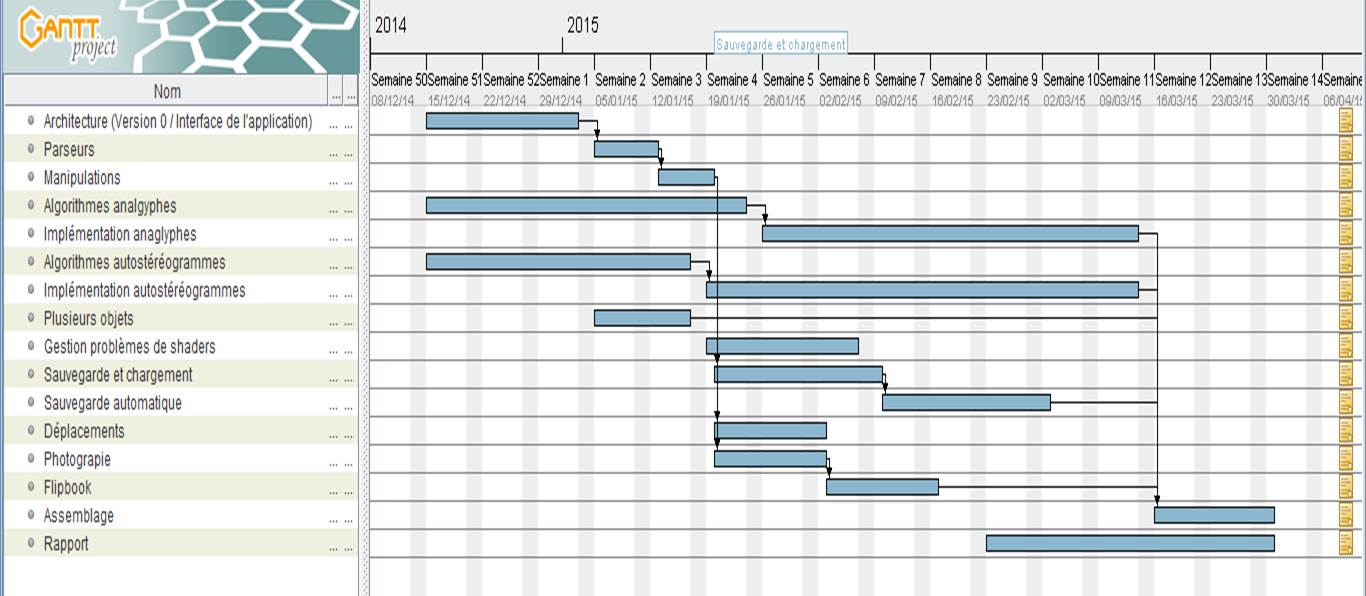
\includegraphics[scale=0.42]{graphGantF.jpg}
        \end{sideways}
	\caption{\label{fig:graphGantF} Graphe temporel du déroulement du projet \protect \footnotemark }
\end{figure}
\footnotetext{Réalisé grâce au logiciel GanttProject : http://www.ganttproject.biz/}

\begin{figure}[h]
	\centering
	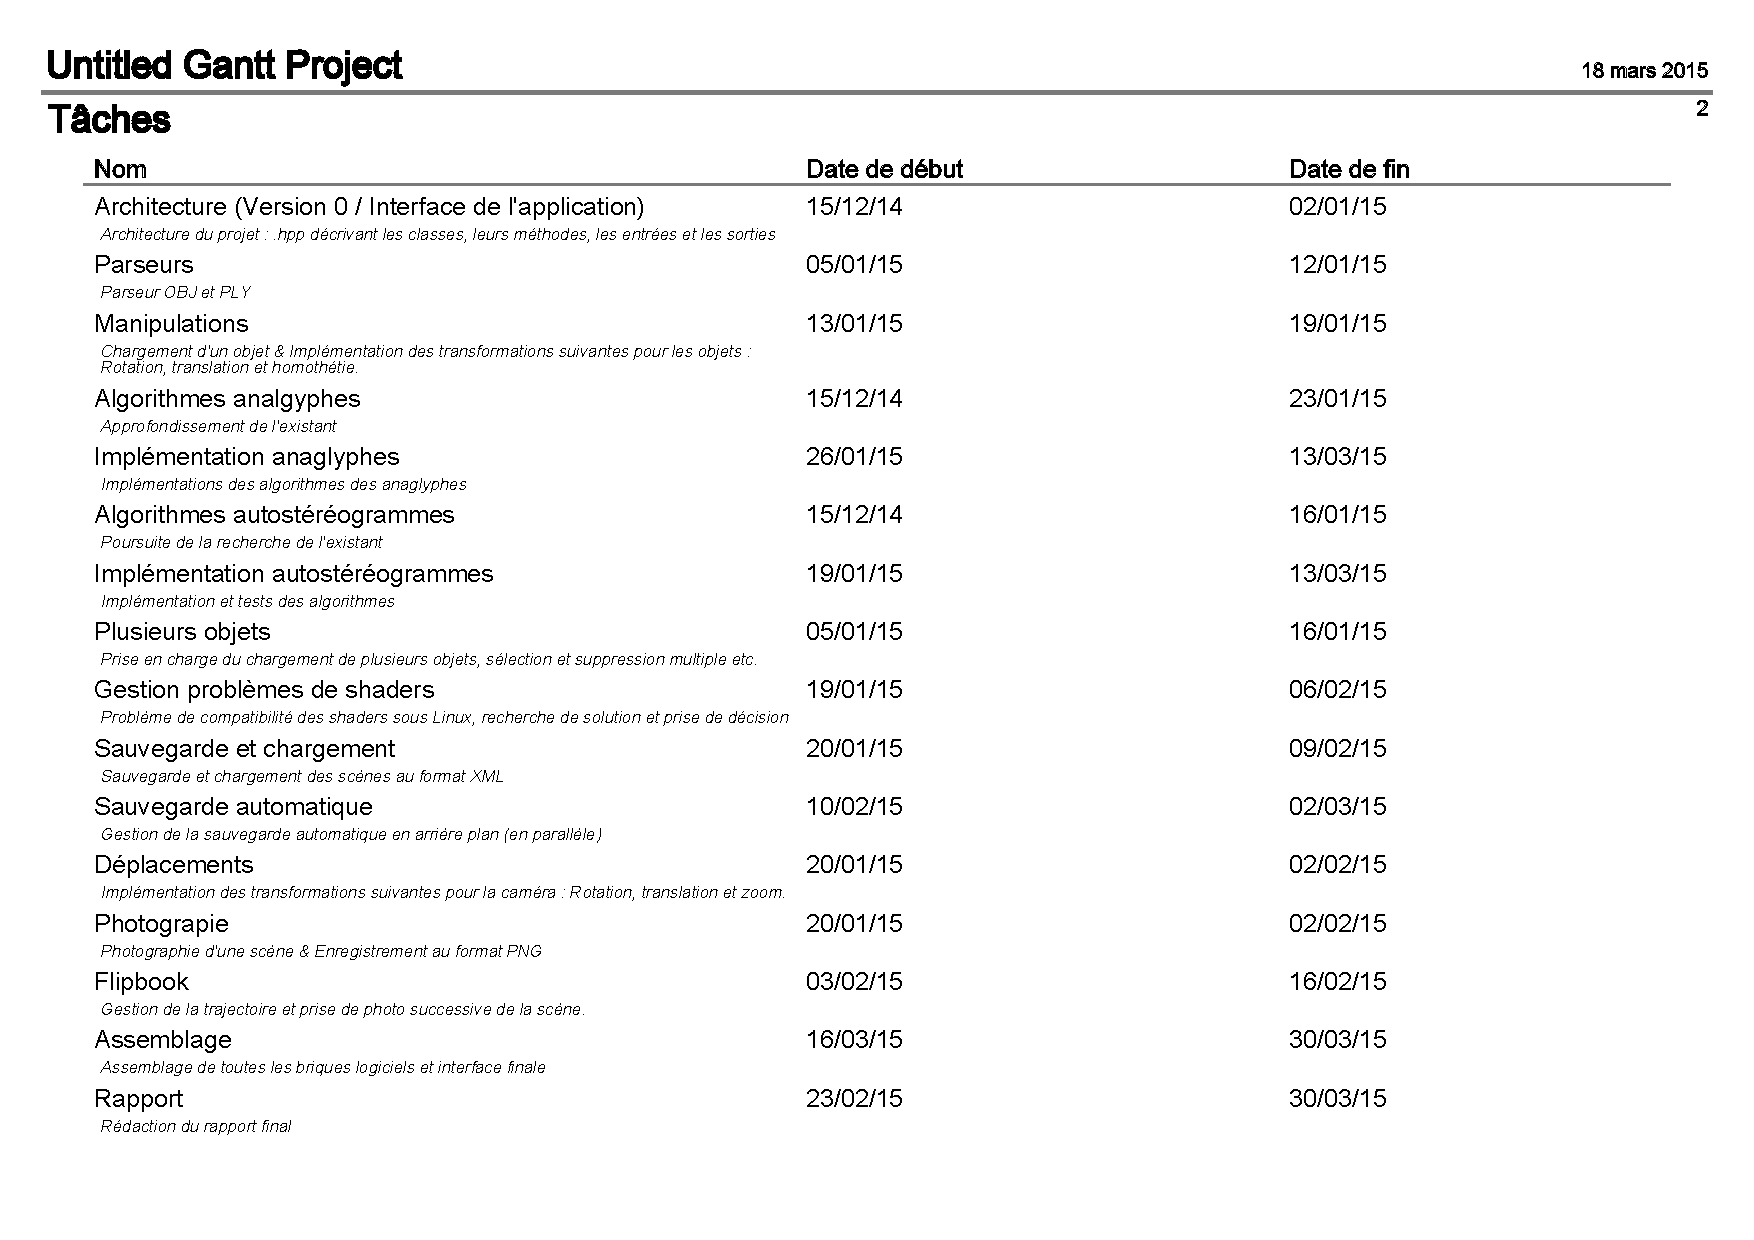
\includegraphics[scale=0.6]{gantf.pdf}
	\caption{\label{fig:gantF} Récapitulatif des tâches et des périodes par tâche \protect \footnotemark }
\end{figure}
\footnotetext{Réalisé grâce au logiciel GanttProject : http://www.ganttproject.biz/}

\paragraph{}
Les principales modifications consistent ainsi dans l'allongement de la période destinée à la recherche d'algorithmes pour les rendus et à leur implémentation et dans la réorganisation chronologique des tâches. Les raisons de ces différences ont été expliquées précédemment, notamment dans la partie Difficultés rencontrées.
Les manipulations des objets et de la scène ont été effectuées plus rapidement que prévu, mais une période de retour en arrière à cause des shaders a été ajoutée, allongeant la période de travail sur le chargement et la sauvegarde de la scène qui a été momentanément interrompu le temps de régler ce problème.

\paragraph{}
Malgré ces débordements dans le temps, la réalisation du projet se sera achevée dans les temps, le dernier mois ayant permis d'intégrer les algorithmes au logiciel, de compléter et de parfaire des fonctionnalités.

Au final, l'ensemble des manipulations de la scène et de ses objets qui avaient été promises dans le cahier des charges ont été implémentées. De même, l'ensemble des rendus prévu est générable à partir de la scène, deux algorithmes de génération sont proposés pour les autostéréogrammes et trois pour les anaglyphes.

\paragraph{}
Au niveau des besoins non fonctionnels, la portabilité aura été respectée malgré l'utilisation des shaders qui auraient pu poser problème sur certaines machines. Grâce aux nombreux modules proposés par la bibliothèque Qt, portable et très complète, des solutions auront été trouvées pour l'ensemble des modules et des cas d'utilisation sans avoir à sacrifier de fonctionnalité pour permettre l'utilisation du logiciel aussi bien sous Windows que sous Linux.

\paragraph{}
Bien que l'indication ne soit pas donnée dans le logiciel, l'utilisation de Project3Donuts en parallèle de l'utilisation du logiciel Fraps\footnotemark nous a permis de vérifier la fluidité du logiciel. Grâce notamment aux modèles 'happy.ply' et 'blade.ply' présentés dans le cahier des charges, les valeurs de frames par seconde données dans le cahier des charges ont été validées.
\footnotetext{\url{http://www.fraps.com/}}
\paragraph{}
Enfin, la maintenabilité du logiciel sera également possible grâce au choix des outils et à l'architecture du projet. 
Tout d'abord, l'utilisation de Qt5, qui est actuellement la plus récente version de Qt, laisse envisager que le logiciel pourra être utilisé longtemps sans avoir à migrer vers une nouvelle version de la bibliothèque. Ensuite, l'utilisation de OpenGL ES 2.0, qui est la version d'OpenGL de base avec Qt5, pourrait éventuellement permettre de générer une application mobile du logiciel. 
L'architecture a également été pensée pour permettre cette maintenabilité. En effet, la présence des différents rendus et de plusieurs algorithmes pour chaque rendu montre bien qu'il est aisé d'en ajouter de nouveau.

\paragraph{}
Ce bilan positif montre que l'ensemble des besoins fonctionnels et non fonctionnels ciblés dans le cahier des charges ont été implémentés avec succès. Nous espérons que ce projet sera réutilisé et maintenu, puisqu'il a été conçu dans cette optique. Il sera éventuellement possible de créer une application mobile à partir du code existant, ou d'ajouter et de tester d'autres algorithmes ou d'autre rendus possibles à partir d'une scène en trois dimensions. Nous espérons également que nos clients auront été satisfaits du travail réalisé et du logiciel final. 

\paragraph{}
Malgré la réussite globale du projet, l'exercice du PFA aura présenté quelques difficultés dans la gestion de projet.

\paragraph{}
Dès le début de la période de réalisation, nous devions déterminer les durées et l'ordonnancement des tâches au cours du projet. Grâce à la réflexion apportée par le cahier des charges, il a été toutefois plus aisé de connaître les tâches priotaires et de les estimer. Bien que nous ayons essayé de planifier notre temps en fonction de nos autres obligations à l'école, certaines semaines ont été plus fructueuses que d'autres et nous aurons permis d'avancer plus vite que prévu. A l'inverse, des imprévus, des difficultés de compréhension ou encore des retours en arrière nous ont retardé à d'autres moments.

\paragraph{}
Travailler dans une équipe nombreuse aura été bénéfique pour notre apprentissage de la gestion de projet. En effet, habitués dans le cadre de nos études à réaliser des projets par équipe de trois ou quatre, la répartition des tâches et la place de chacun dans l'équipe est plus facile à trouver. Dans une équipe de sept personnes, chaque tâche est répartie entre plusieurs personnes, et chacun doit faire sa part dans chaque tâche. Les rythmes de travail étant différents, cette expérience nous a montré à quel point il est important que chacun ait son rôle, sa place, pour qu'il puisse avancer à son rythme.

\paragraph{}
Enfin, l'implémentation de ce projet a été réalisée dans un contexte de méthode agile. En effet, chaque semaine, nous pouvions faire le point avec nos clients de l'avancée du projet, et leurs remarques nous permettaient d'une semaine à l'autre de revenir sur le logiciel. Cette méthode de développement permet d'avoir des objectifs sur de petites périodes et de pouvoir se rendre compte de l'éventuel retard pris sur le produit final. Elle permet également de s'assurer de la satisfaction des clients, puisque ceux-ci ont eu à plusieurs reprises l'occasion de voir l'avancée du logiciel, de pouvoir le tester et éventuellement de nous demander des corrections. Cette méthode de développement agile permet donc d'avancer plus sereinement au fil du projet, en ayant conscience du travail qu'il reste à fournir et en s'assurant de la satisfaction des clients.
